% chktex-file 1
% chktex-file 13

\subsection{Distributed File Sharing}
\label{subsec:design-p2p}

This section will look at how various types of game data can be shared across a distributed set of peers using a content-addressable hash tree to describe the data.  

\subsubsection*{Hash Tree}
\label{subsubsec:hash-tree}

The hash tree of a given directory is used to represent its structure as well as the contents of its files. Each file is represented by an ordered list of SHA-256 hashes that match a fixed-size block of data. This allows users to easily identify and verify game data \reqref{F-M10}. Users should be able to specify which folders/files to exclude when generating a hash tree.

\begin{figure}[ht]
  \centering
  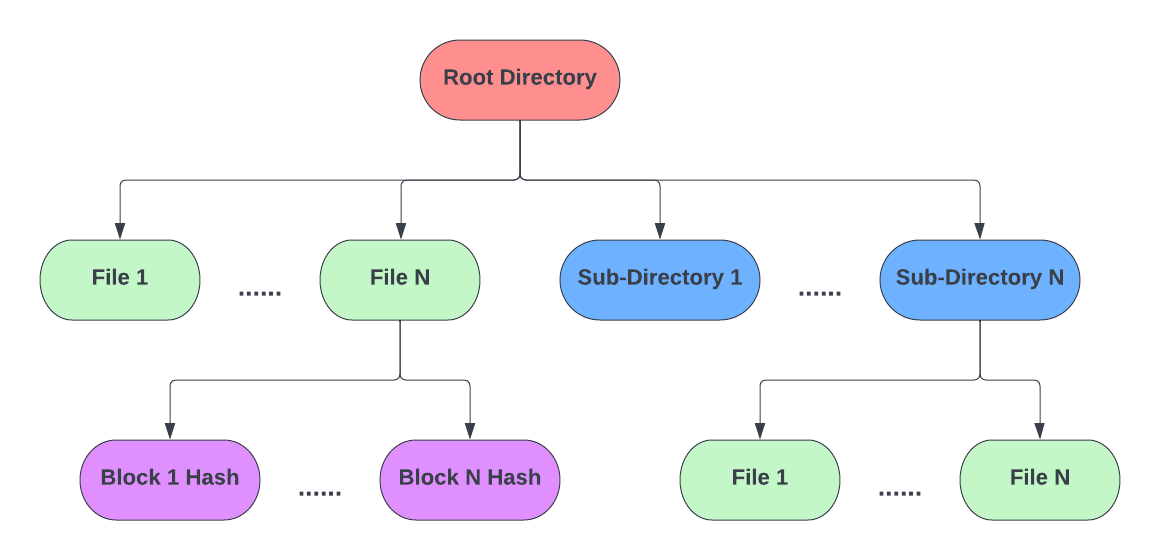
\includegraphics[width=.85\textwidth]{assets/images/diagrams/block-body.png}
  \caption{The structure of a hash tree}
  \label{fig:hash-storage}
\end{figure}

\newparagraph
Hash trees will be stored on IPFS with the CID being kept with the other game metadata on Ethereum.

\subsubsection*{Downloading Content}

\newcommand{\seeder}{$P_{seeder}$~}
\newcommand{\downloader}{$P_{downloader}$~}

Games are content addressable using their root hash field, which will allow users to request data from that game from other users. When a peer seeking data \downloader forms a connection with another peer \seeder they will:

\begin{enumerate}
  \item Perform a handshake to determine each other's Ethereum address and public key.
  \item \downloader will send requests for individual blocks to \seeder \reqref{F-M9}.
  \item Upon receiving the first request, \seeder will verify that \downloader owns the game by checking the \textit{purchased} mapping on the smart contract \reqref{F-M6} \reqref{F-S1}.
  \item Upon receiving a block, \downloader will verify the contents using the block's hash \reqref{F-M10} before writing it to disk in the appropriate location.
  \item Repeat Steps 3--4 until the entire game has been downloaded \reqref{F-M11}.
  \item \seeder may request a signed receipt that details the blocks they uploaded \reqref{F-S3} to \downloader.
\end{enumerate}

\newparagraph
Users will be able to connect and send requeststo many peers at once \reqref{F-M7}. Requests will be sent in a round-robin fashion to evenly distribute the requests and prevent overloading a single peer \reqref{NF-S1}. Requests that cannot be completed will be retried when connecting to a new peer or when a peer has a change in library.

\subsubsection*{Updating Content}\label{subsubsec:updating}

To satisfy \reqref{F-M2}, developers will upload the game and also provide the root hash of the most previous version of the game, where only the original uploader will be allowed to publish an update to an existing game \reqref{NF-M5}. Any users who own a previous version of a game will be allowed access to all future versions \reqref{F-M3}.
\x
Each version is considered its own game and will require users to download the updated version separately. Whilst this isn't reflective of how updates are typically managed, this will be acceptable for the scope of this project.

\subsubsection*{Downloadable Content}

Downloadable Content (DLC) \reqref{F-C1} represent optional additions for games that users will buy separately. DLCs will act similarly to how updates are treated. Each DLC will need:

\begin{enumerate}
  \item \textbf{Dependency} The root hash of the oldest version of the game this DLC supports.
  \item \textbf{Previous Version} (Optional) The root hash of the previous version of the DLC.
\end{enumerate}

\newparagraph
Users must own the original game to buy any of its DLC. 

\subsubsection*{Proving Contribution}

As a user downloads blocks of data, they will keep track of which users have sent them which blocks. A peer may then request their contributions in the form of a signed message that can be sent to the developer \reqref{F-S3} in return for some kind of reward. The contents of the reward isn't specified for this project but could include in-game items, digital assets or Ether. This solution assumes that developers have knowledge of which Ethereum address maps to which of their game's users.